\documentclass[10pt,conference,compsocconf]{IEEEtran}
\usepackage{comment}
\usepackage{hyperref}
\usepackage{graphicx}	% For figure environment
\usepackage[font=small,skip=0pt]{caption}

\begin{document}
\title{Finding the Higgs Boson \\ Machine Learning Project 1}

\author{
  Carlos Meg\'ias, Jorge S\'anchez and Roser Vi\~nals\\
  \textit{\'Ecole polytechnique f\'ed\'erale de Lausanne, Switzerland}
}

\maketitle

\begin{abstract}
  Machine learning (ML) has become a key enabler for the analysis and classification of data. In this project, a CERN's database has been used to create a model for predicting whether a decay signature of a collision event represented by a vector of features was signal (a Higgs boson) or background (something else).
  
\end{abstract}

\section{Introduction}
This report has been divided in five sections. Section \ref{sec:FeatureProcessing} presents the different techniques considered for feature preprocessing in order to deal with the CERN's data set particularities. Concerning the predictive model, Section \ref{sec:Model selection} justifies how the hyperparameters and the cost function have been selected. Section \ref{sec:Results} presents and analyses the results obtained, and Section \ref{sec:Summary} concludes the report.
\section{Data Preprocessing}
\label{sec:FeatureProcessing}

In this section, we describe the feature processing techniques implemented. First, the main challenge faced is how to deal with -999 values, which correspond to features of some data points that are meaningless or cannot be computed. We have studied different techniques: a) standardizing each feature (considering the -999 values); b) changing the -999 values by the mean of the others values of each feature (each column); c) changing these values by zeros; d) removing every entry (row) which have a -999 value in at least one of its features; e) and removing each feature which has at least one -999 value in a entry.
For choosing the best technique, we have measured the MSE (Mean Squared Error) and achieved accuracy, defined as the percentage of success, using the Least Squares method as shown in Figure \ref{fig:Data Preprocessing}. Thus, we checked that the best results are obtained when using technique b), as in terms of MSE as of accuracy (which are obviously strongly correlated since when decreasing the error the accuracy should increase). As the -999 are missing values, it seems more suitable replacing these values by the means than removing a huge amount of data (as done in d) and e)), since this would imply the discard of data that could be useful for creating a more reliable model.
From these results, we decided to use technique b). However. once the final model was selected we improve the feature processing. As explained in section \ref{sec:Results}, the best result was obtained when combining option b) with standardization and outliers removal.
\begin{figure}
  \centering
    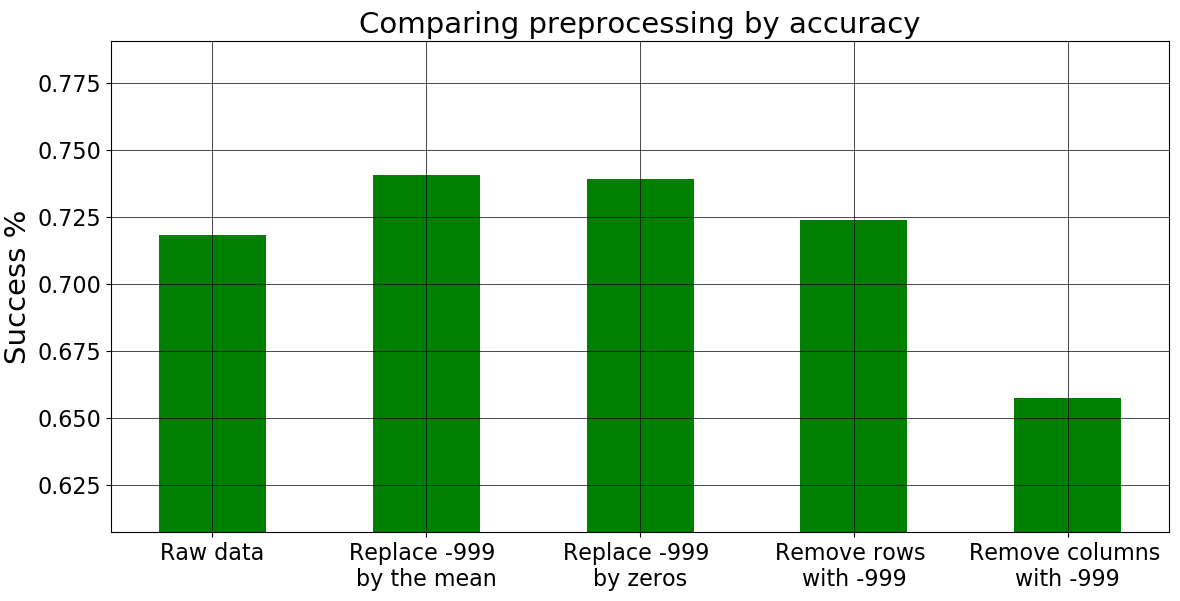
\includegraphics[scale=0.26]{Preprocessing_bar_plot}
    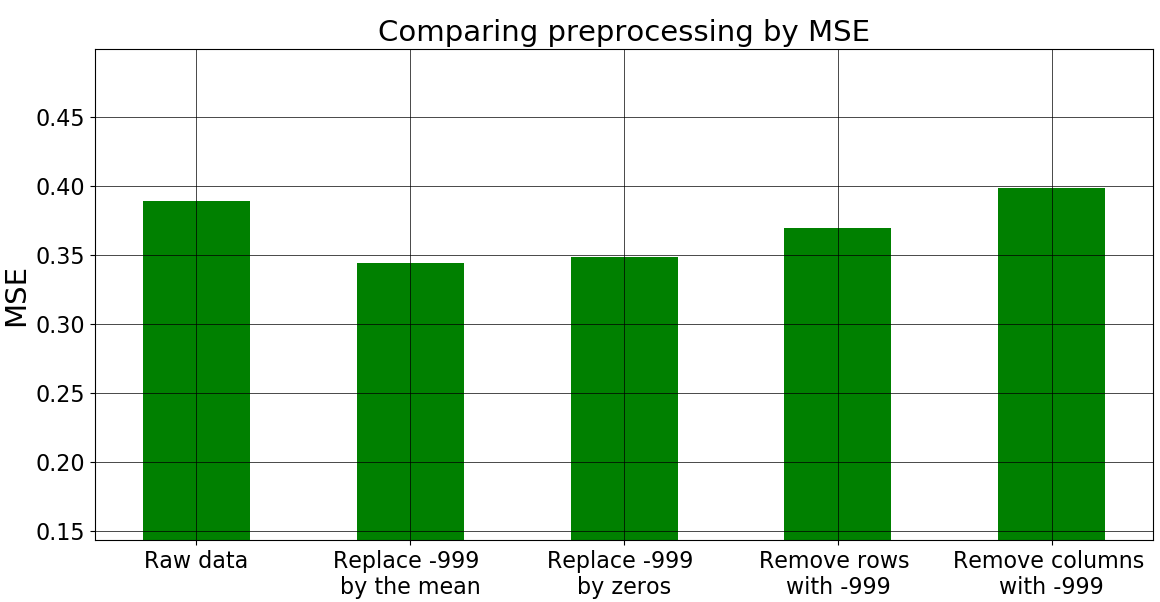
\includegraphics[scale=0.27]{Preprocessing_bar_plot_mse.png}
  \caption[b]{\protect\label{fig:Data Preprocessing}Feature processing techniques considered}
  \setlength{\belowcaptionskip}{-1pt}
\end{figure}
\section{Model selection}
\label{sec:Model selection}
In this section we describe the criteria and final choices that we have used for obtaining our results.
%%¿NO PARECE MÁS LÓGICO EL SIGUIENTE ORDEN?: 
%%A)METHOD SELECTION B)SELECTION CRITERIA C)HYPERPARAMETERS SELECTION
%%SOB

\subsection{Method selection}
\label{selection}
 \begin{enumerate}
    We have considered  two cost functions: the Mean Absolute Error (MAE) and MSE. We have selected the MSE since penalizes large errors.
    On behalf of the method, after comparing the different techniques implemented such as Least squares (with or without gradient descent), ridge regression and logistic regression, we could observe that the method which was achieving higher performance was ridge regression. This performance has been quantified using the criteria described in subsection \ref{selection_criteria}.  
    
 \end{enumerate}
 
\subsection{Selection criteria}
\label{selection_criteria}
 \begin{enumerate}
    
     \item \textbf{Minimum error or maximum accuracy selection}: 
     When searching the optimum weights for building our predictive model we aim minimizing the cost function (as explained in \ref{selection}, the MSE). However, it may not be the best idea using this criteria for comparing models which are already built; in this case what makes the most sense is to decide which model is better checking the accuracy that the models have achieved, since this indicates its predictions quality, rather than checking the MSE. After trying both options, we concluded that taking the maximum accuracy was leading us to better results.
      \item \textbf{Cross-validation}\label{cross}: In order to estimate the error for different models and select the best, we have used one k-fold cross validation. This technique achieves a good compromise between having an unbiased estimate of the generalization error and variance, and a reasonable computation time. Figure \ref{fig:Cross-validation}  shows for different number of partitions, the estimated performance in terms of accuracy and MSE and the computation time required for a fixed model. Since the error estimations does not fluctuate a lot when changing the number of partitions, we have selected a not very high \textit{K} value, \mathrm{\textit{K}=6.}

     
 \end{enumerate}
\begin{figure}
  \centering
   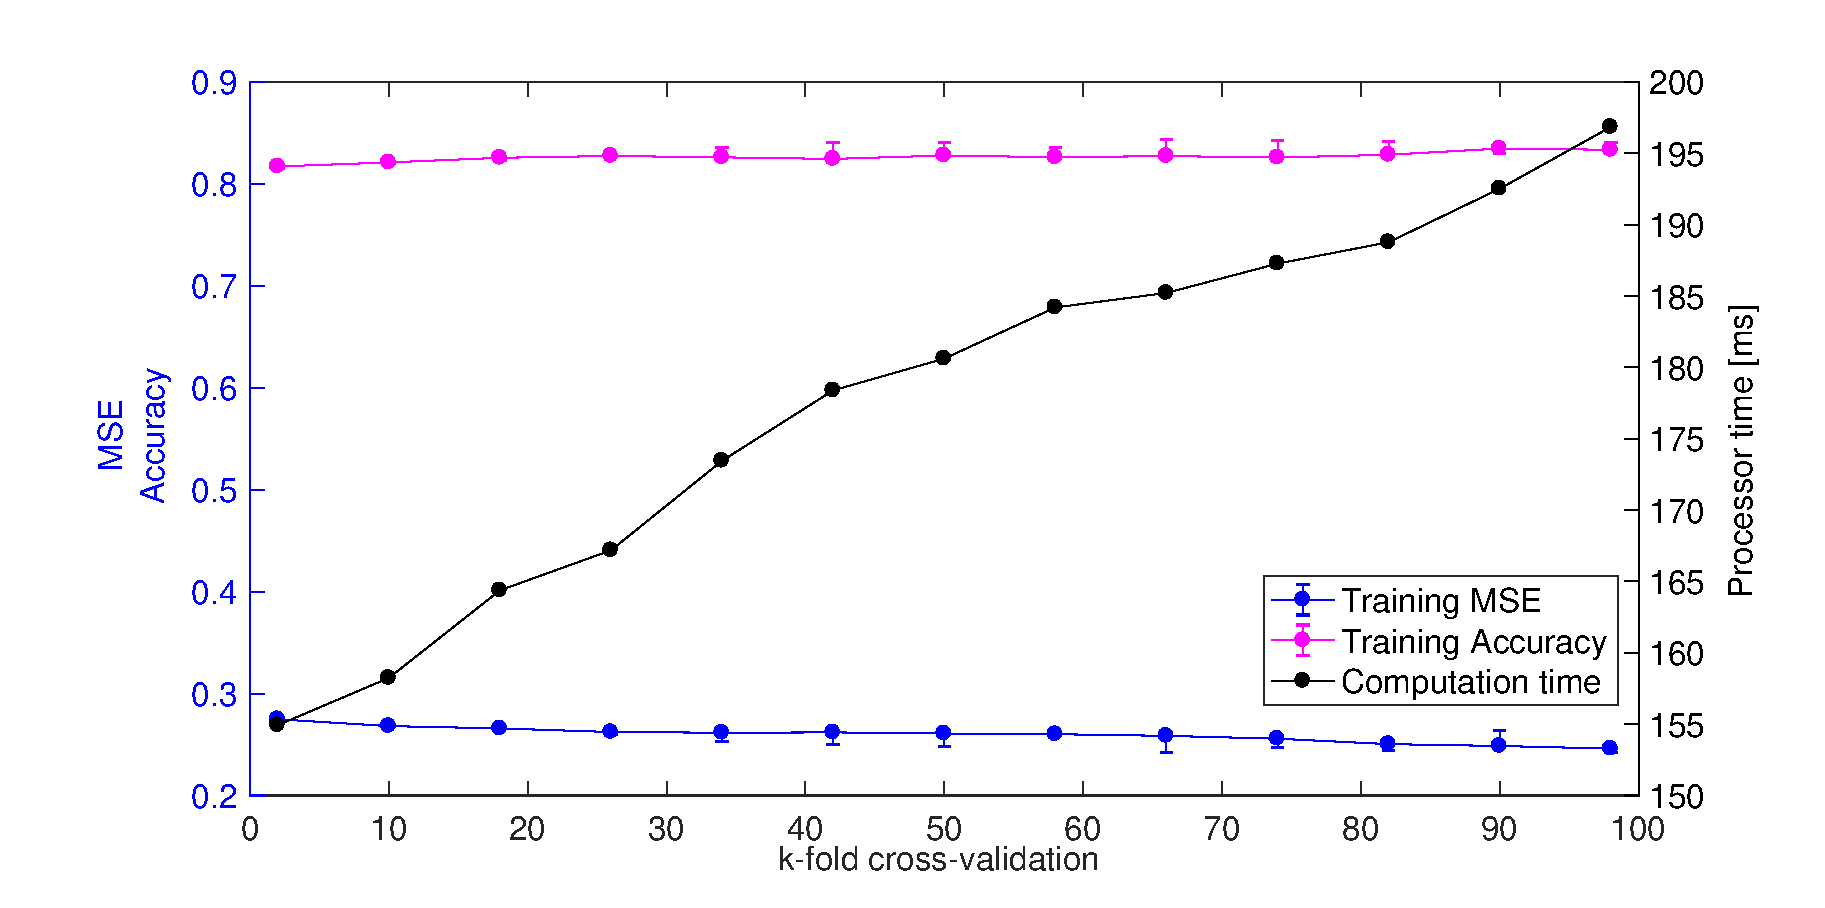
\includegraphics[scale=0.3]{firstk.eps} 
  \caption[a]{\protect\label{fig:Cross-validation}Cross-validation estimation of MSE, accuracy (mean, maximum and minimum) and computation time for ridge regression with $degree=\mathrm{10}$ and $\lambda=\math{10^{-6}.}$}
  \setlength{\belowcaptionskip}{-1pt}
\end{figure}

\subsection{Hyperparameters selection}
 First, we have included the polynomial expansion technique. Different implementations for the polynomial expansion have been developed and compared (included in the code) in order to get a different representation of the data that could lead us to better results. The result of applying a determined \textit{degree} polynomial to each feature is a set of new entries with $degree\times Num Original Features$ features. In order to perform this proceadure, the polynomial \textit{degree}, which is our first hyperparameter, needs to be determined in order to get the best model.
 
 \begin{figure}
  \centering
   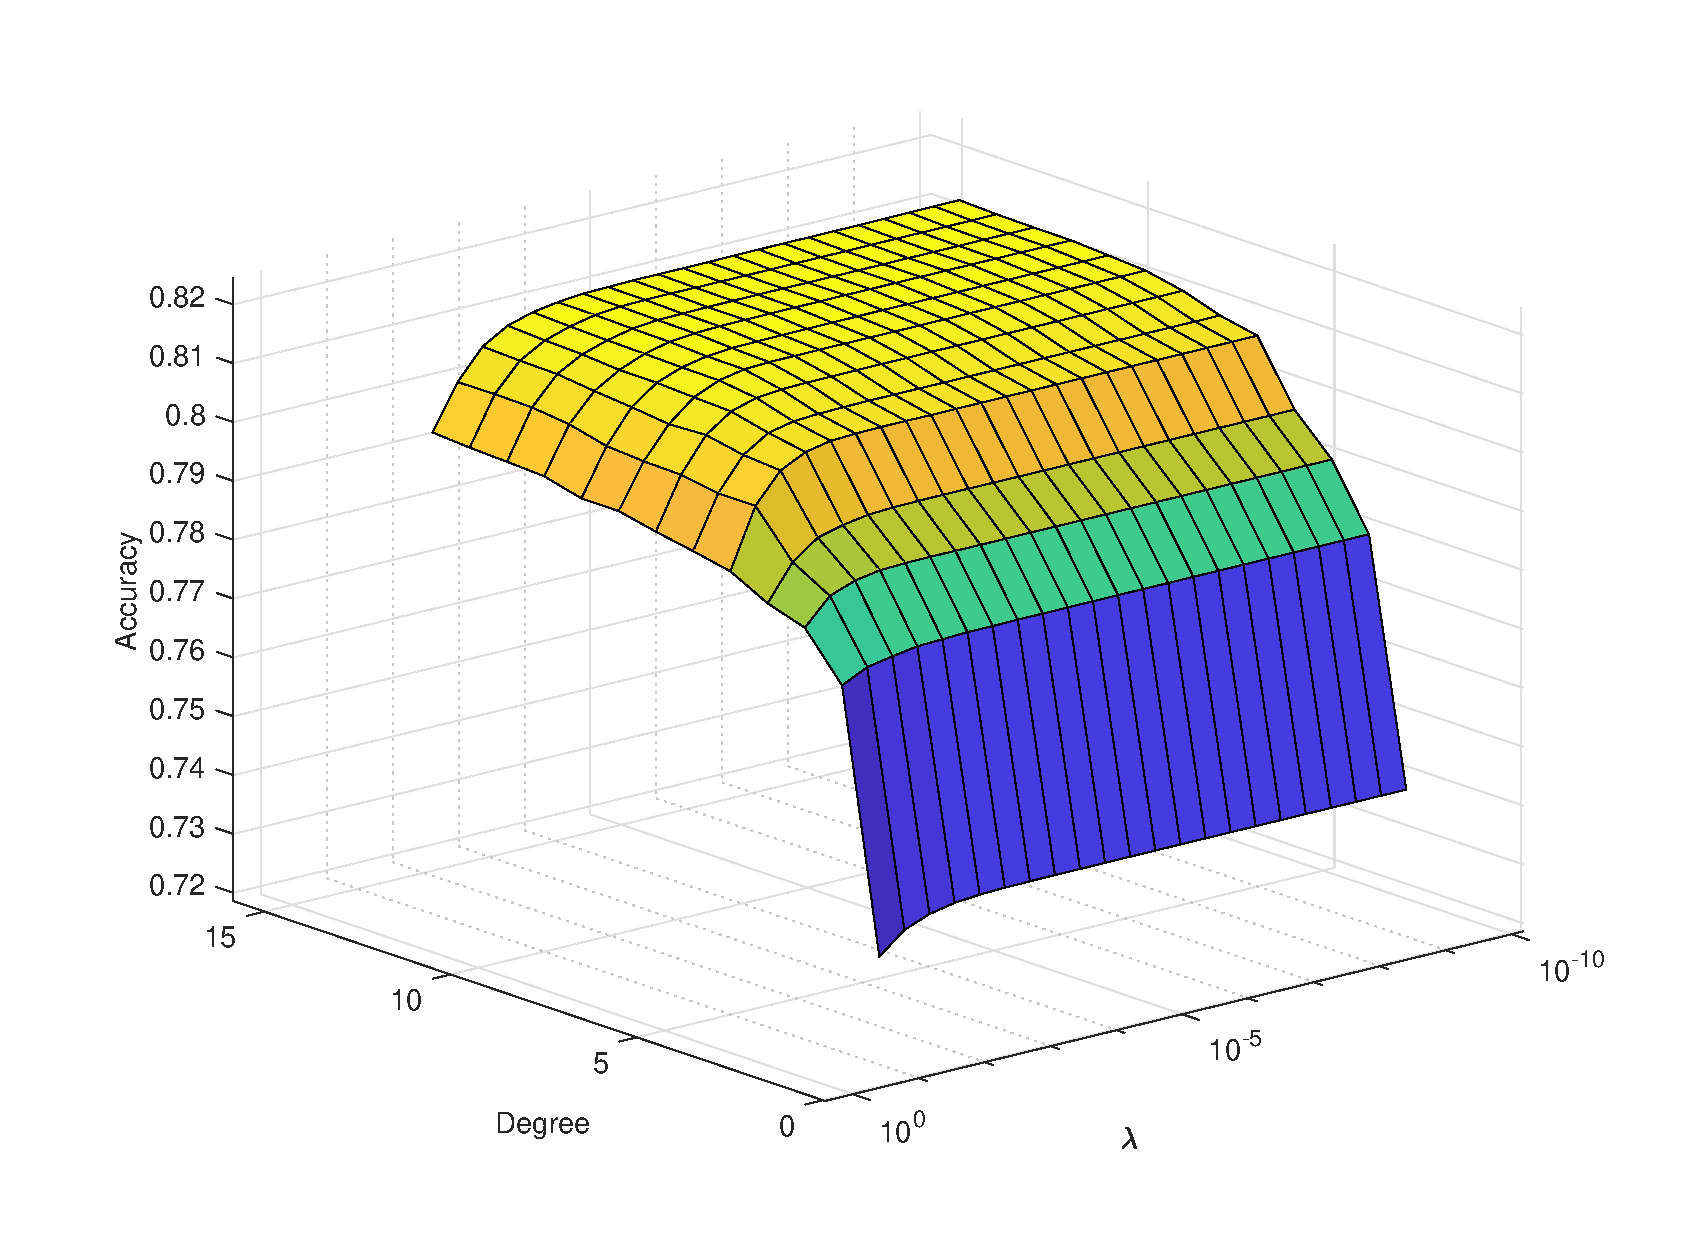
\includegraphics[scale=0.3]{acc.eps} 
  \caption[c]{\protect\label{fig:hyper}Hyperparameter selection: $degree=11$ and $\lambda=3.73\times10^{-5}$}
  \setlength{\belowcaptionskip}{-1pt}
\end{figure}
Second, for ridge regression, another hyperparameter is required:  $\lambda$. This hyperparameter adjusts the regularization for preventing overfitting. The regularization used is L2-Regularization which takes the euclidean norm of our weights vector. For the selection of the two best  hyperparameters, we first explored a wide range of possibilities and then, we have narrowed down this range until the final values were selected. Using k-fold cross validation (see \ref{cross}), we have iterated over the different ranges and we have obtained the results in Figure \ref{fig:hyper}. We see that the accuracy reaches the maximum when $degree=11$ and $\lambda=3.73\times10^{-5}$, the same values than the ones used for the Kaggle's submission. 

 
\section{Results}
\label{sec:Results}
The final results have been obtained after applying the preprocessing techniques described in Section \ref{sec:FeatureProcessing}. We have first removed the -999 values and replaced them by the mean of the corresponding features. Afterwards, the data has been standardized. After the standardization, the outliers have been removed by setting a threshold in -5 and 5, i.e. the features whose values are bellow -5 or above 5, have been replaced by 0. This threshold could have been optimally selected by computing the best one for each feature. However, for simplification, we considered the same threshold for all the features and we just tried few values in the range between 1 and 7. The better performance was achieved when taking 5. 

By iterating over a wide range of values of the two hyperparameters considered, and taking the ridge regression with the MSE function, the model has been selected and tested. The achieved accuracy is 0.8173 in the Kaggle's submission. It is important mentioning that the best results have been obtained when:
\begin{enumerate}
    \item Replacing the unmeasured values (-999) by the corresponding means, standardizing the data and removing the outliers by setting a threshold.
\item Using k-cross validation. For computation reasons, we have used 6 partitions.
\item Using ridge regression to minimize the MSE has led us to better performance than other techniques such Least Squares or Logistic regression.
\item The hyperparameters selection has been critical. A wide range was considered initially and has been narrowed until the optimal values were selected. 
\end{enumerate}


\section{Summary} %What to write in this section?
\label{sec:Summary}
In this project, we have developed a classifier that predicts whether a collision event has occurred or not. We have shown that the choice of the feature preprocessing technique and the hyperparameter selection is critical. The best performance was achieved when we using 6-cross validation and ridge regression technique for computing the weights with $degree=11$ and $\lambda=3.73\times10^{-5}$, achieving a final accuracy of 81.784\%.

\bibliographystyle{IEEEtran}
\bibliography{literature}

\end{document}
